\documentclass[12pt]{article}

\title{A numerical, visual method for generating the (non-)linear separating isosurface of two classes of objects in two-dimensional space using Marching Squares and OpenCV}
\author{
Shawn Halayka\footnote{Independent -- sjhalayka@gmail.com}
}


\date{\today\;\currenttime}

\usepackage{datetime}
\usepackage{listings}
\usepackage{cite}
\usepackage{xcolor}
\usepackage{graphicx}
\usepackage{setspace}
\usepackage{amsmath}
\usepackage{url}
\usepackage{amsfonts}
\usepackage{caption}
\usepackage{subcaption}

\usepackage[margin=1in]{geometry}

%\doublespace

\begin{document}




\maketitle

\begin{abstract}
With regard to the separating isosurface of two classes of objects in two-dimensional space, the transition from rectilinear to curvilinear is documented.
Marching Squares and OpenCV were used to calculate the data that were used for illustrations in this paper.
It is found that the curvilinearity is adjustable via variable grid resolution, as well as via convolution such as Gaussian blur.
\end{abstract}




\section{Introduction}

In terms of statistical learning, a balance between high variance (curvilinearity) and high bias (rectilinearity) is to be had \cite{james}.
However, it is not clear from \cite{james} how to go about obtaining a nonlinear, radial isosurface without having to rely on the Support Vector Machine (SVM) functionality in the popular R library e1071.
Thus, it can be daunting to those wishing to perform such a thing from the ground up in other languages, such as C++ or Python.

The goal of this paper is three-fold: 1) to pay homage to \cite{james}, and 2) to have fun, as well as 3) to show that obtaining such an isosurface is a simple matter, especially so when there are only two classes and they are in only two-dimensional space.

The images passed into the Marching Squares algorithm give our technique an inherent visual property.
Simply put: Marching Squares \cite{halayka, gong, bobrowski} works as a radial (spherical) isosurface generator, as well as a rectilinear (planar) isosurface generator -- it all depends on the grid resolution.
The data generated by Marching Squares are the line segments that separate the two classes, as well as triangles for the area of each class.
Classifying a test point is a matter of ray-triangle intersection, which can be accelerated using a Bounding Volume Hierarchy or quadtree data structure.

OpenCV \cite{opencv} was used to downsize images, as well as blur images.
OpenCV could also have been used to sharpen images, etc.
There are many convolutions to experiment with.

Please see \cite{halayka} for a small introductory Marching Squares code in C++.





\section{Regarding the illustrations}

Fig. 1 shows a 2x2 pixel bitmap image.
This image's pixel values are used as input to the Marching Squares algorithm.
The output of the Marching Squares algorithm is shown in Fig. 2 -- a rectilinear separation is produced.

Figs. 3 and 4 show the same points, but with a 16x16 pixel image -- a rough, curvilinear, radial separation is produced.

Figs. 5 and 6 show the same points, but with a 64x64 pixel image -- a smooth, curvilinear, radial separation is produced.

Figs. 7 and 8 show the contour sets, in transparent grey, generated by batches and batches of training data.
The 2x2 pixel images used to generate these contour sets are then averaged, and the so-called average contour is shown in black.
The result is a rectilinear separation.

Figs. 9 and 10 show the contour sets, in transparent grey, generated by batches and batches of training data.
The 64x64 pixel images used to generate these contour sets are then averaged, and the so-called average contour is shown in black.
The result is a smooth, curvilinear, radial separation.

Figs. 11 and 12 use the same 64x64 pixel image, except that it's been blurred once.
It is apparent that this removes the higher-resolution detail from the isosurface.

Figs. 13 and 14 use the same 64x64 pixel image, except that it's been blurred ten times.
It is apparent that this further removes the higher-resolution detail from the isosurface.

As these illustrations show, the amount of curvilinearity (and thus variance versus bias) is easily adjustable using simple computer vision techniques.




\section{Conclusion}

It is apparent that \cite{james} is a treasure trove of statistical learning techniques, although it does not give many details when it comes to generating a radial isosurface outside of the realm of the SVM.
Here we have illustrated how Marching Squares and OpenCV can be used to generate such a radial isosurface.
This numerical, visual method of generating the (non-)linear separating isosurface of two classes of objects in two-dimensional space is easy to implement, and is as far as we know, novel.

This paper's reference section is rather small, and the hunt for the literature is left to those who have access to the journals.



\pagebreak




\begin{thebibliography}{9}

\bibitem{james} James, et al. An Introduction to Statistical Learning with Applications in R. ISBN: 978-1-0716-1417-4
\bibitem{halayka} Halayka. Marching Squares C++ implementation.\newline \url{https://github.com/sjhalayka/Marching-Squares}
\bibitem{gong} Gong and Newman. A corner feature sensitive marching squares. Southeastcon 2013 Proceedings of IEEE, pp. 1-6, 2013
\bibitem{bobrowski} Bobrowski. Estimation of systematic errors of discrete line approximation by triangular tessellation and marching squares algorithm. Micron, vol. 141, pp. 102966, 2021
\bibitem{opencv} OpenCV library.\newline \url{https://opencv.org/}


\end{thebibliography}



\pagebreak





\begin{figure} 
\centering
  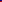
\includegraphics[width = 3 in]{2_res_image.png}
  \caption{Bitmap image used as input to the Marching Squares algorithm.
Image size is 2x2.
}
\end{figure}


\begin{figure} 
\centering
  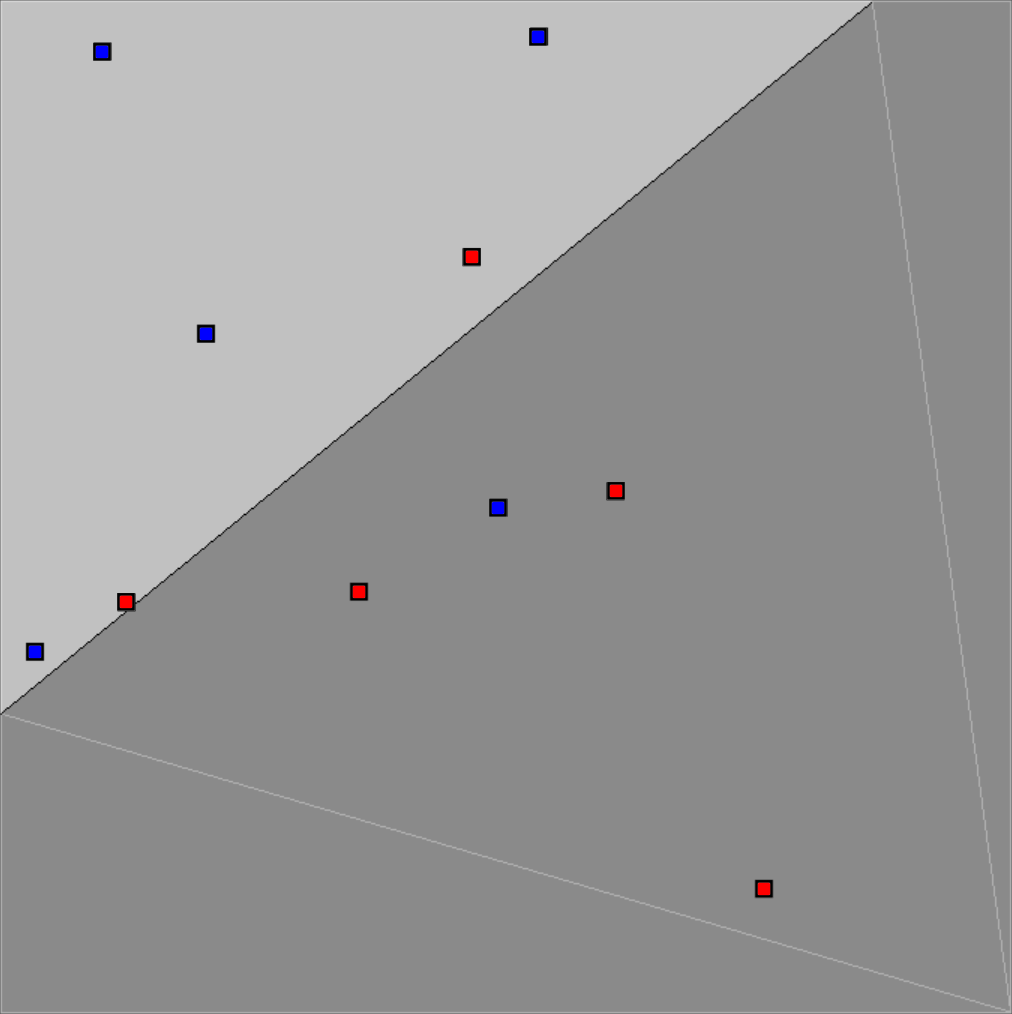
\includegraphics[width = 3 in]{2_res.png}
  \caption{The output of the Marching Squares algorithm: rectilinear separation. Grid resolution is 2x2.
}
\end{figure}






\begin{figure} 
\centering
  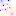
\includegraphics[width = 3 in]{16_res_image.png}
  \caption{Bitmap image used as input to the Marching Squares algorithm.
Image size is 16x16.
Colour falls off with distance.
}
\end{figure}


\begin{figure} 
\centering
  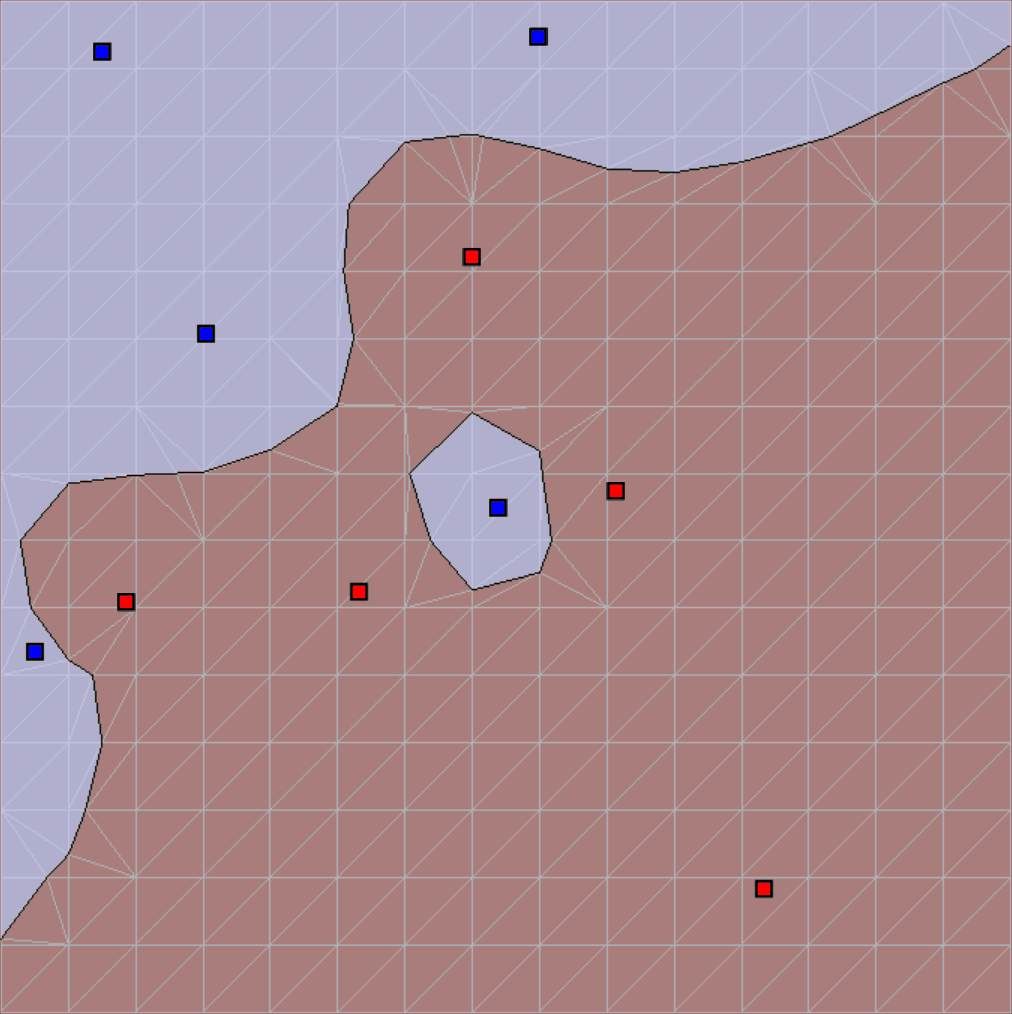
\includegraphics[width = 3 in]{16_res.png}
  \caption{The output of the Marching Squares algorithm: curvilinear, radial separation. Grid resolution is 16x16.
}
\end{figure}



\begin{figure} 
\centering
  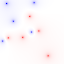
\includegraphics[width = 3 in]{64_res_image.png}
  \caption{Bitmap image used as input to the Marching Squares algorithm. 
Image size is 64x64.
}
\end{figure}

\begin{figure} 
\centering
  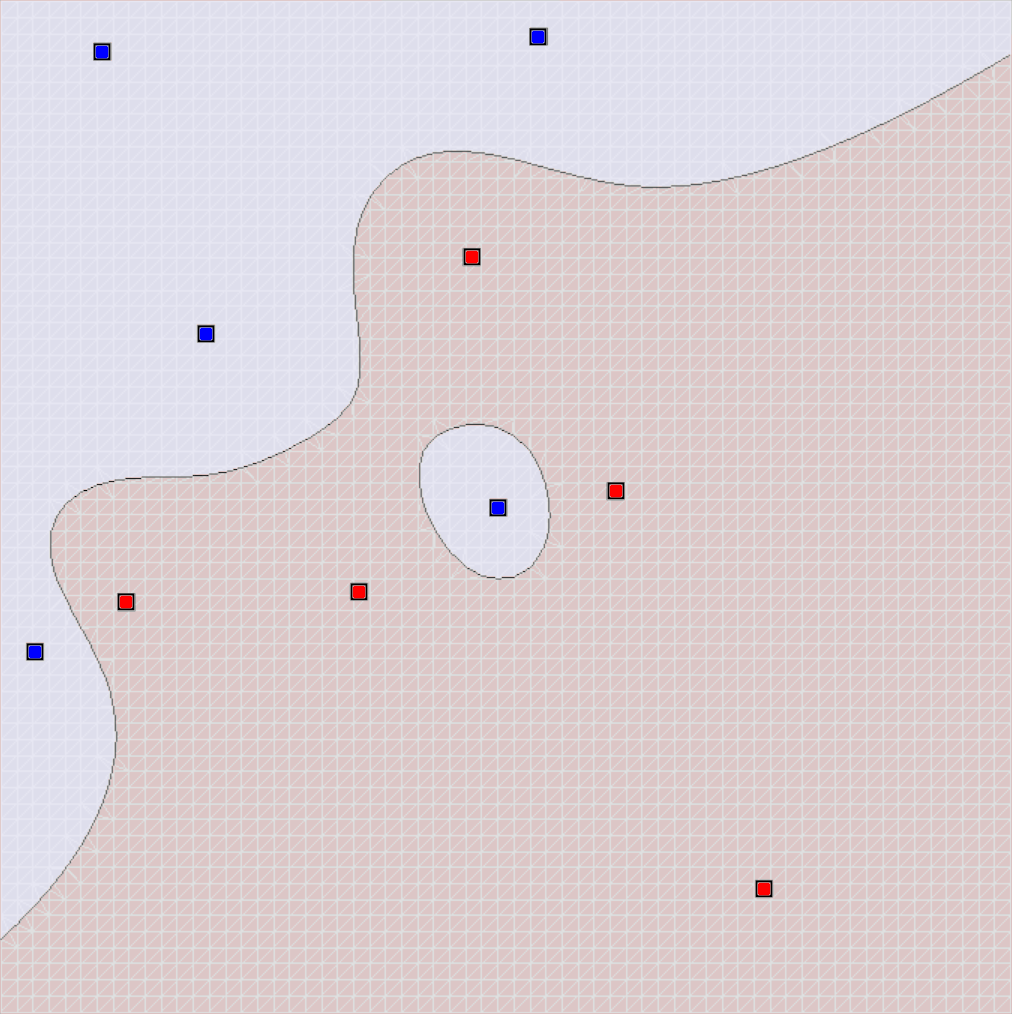
\includegraphics[width = 3 in]{64_res.png}
  \caption{The output of the Marching Squares algorithm: curvilinear, radial separation. Grid resolution is 64x64.
}
\end{figure}







\begin{figure} 
\centering
  
\includegraphics[width = 3 in]{image_avg_rectilinear.png}
  \caption{Bitmap image used as input to the Marching Squares algorithm.
Image size is 2x2.
}
\end{figure}

\begin{figure} 
\centering
  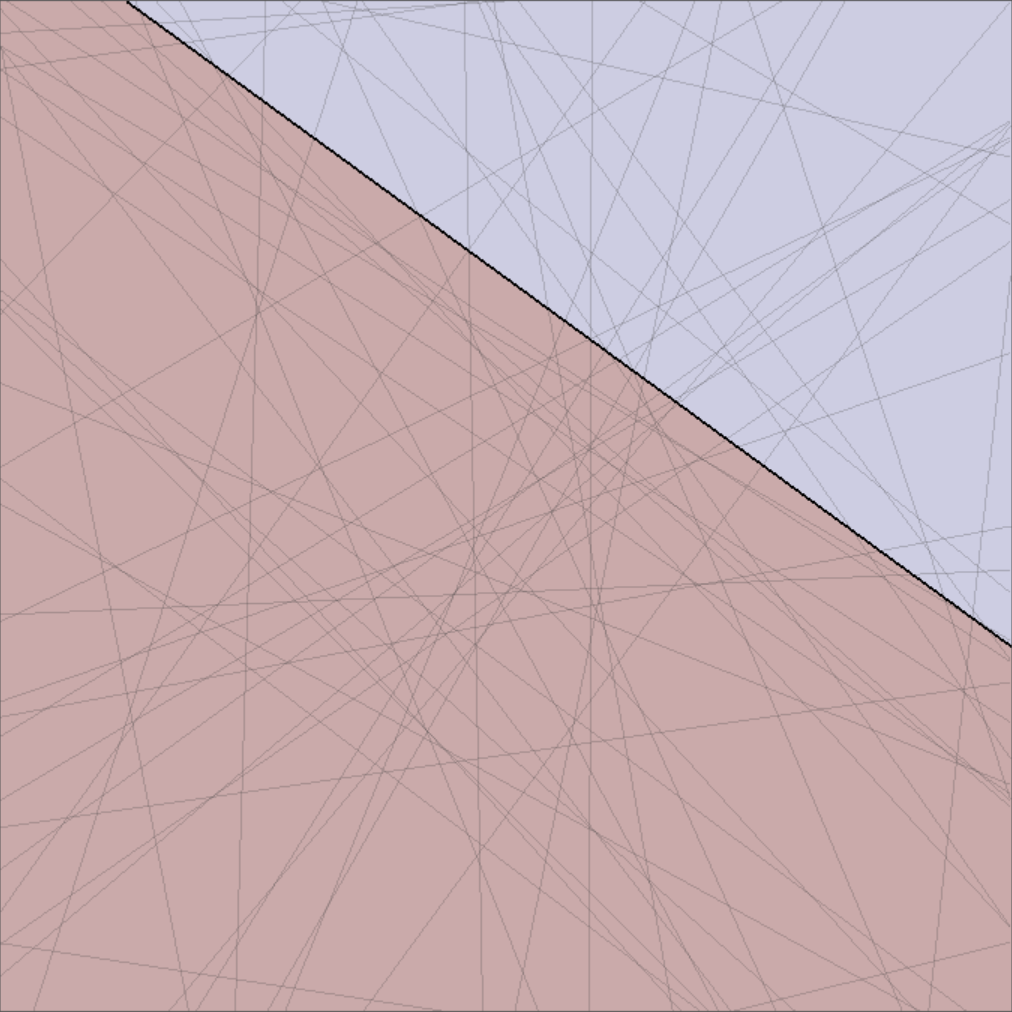
\includegraphics[width = 3 in]{rectilinear.png}
  \caption{The output of the Marching Squares algorithm: rectilinear separation. 
Grid resolution is 2x2.
All contour sets have been drawn in transparent grey, with the exception of the average contour set, which is drawn in pure black.
}
\end{figure}



\begin{figure} 
\centering
  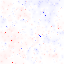
\includegraphics[width = 3 in]{image_avg_no_blur.png}
  \caption{Bitmap image used as input to the Marching Squares algorithm.
Image size is 64x64.
}
\end{figure}

\begin{figure} 
\centering
  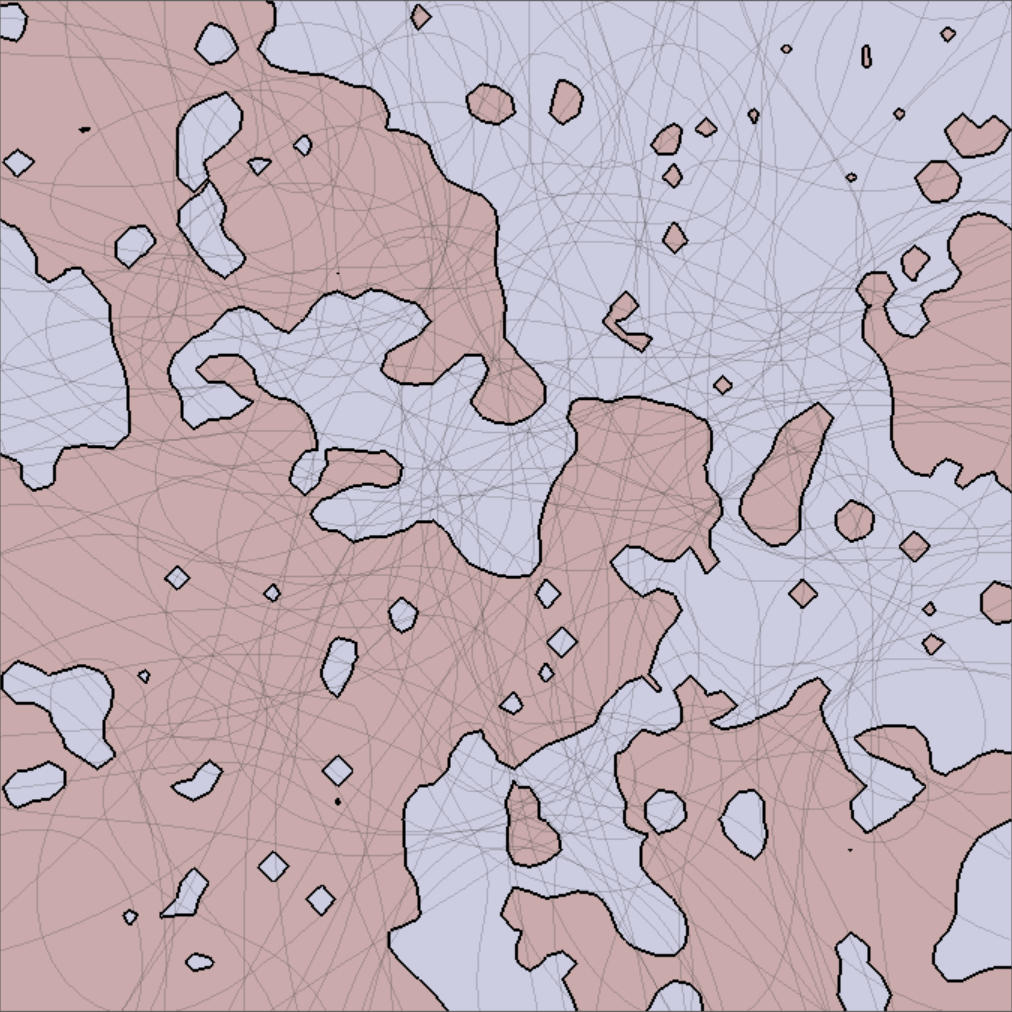
\includegraphics[width = 3 in]{no_blur.png}
  \caption{The output of the Marching Squares algorithm: curvilinear, radial separation. 
Grid resolution is 64x64.
All contour sets have been drawn in transparent grey, with the exception of the average contour set, which is drawn in pure black.
}
\end{figure}





\begin{figure} 
\centering
  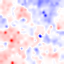
\includegraphics[width = 3 in]{image_avg_1blur.png}
  \caption{Bitmap image used as input to the Marching Squares algorithm.
Image size is 64x64.
One iteration of Gaussian blur has been used.
}
\end{figure}


\begin{figure} 
\centering
  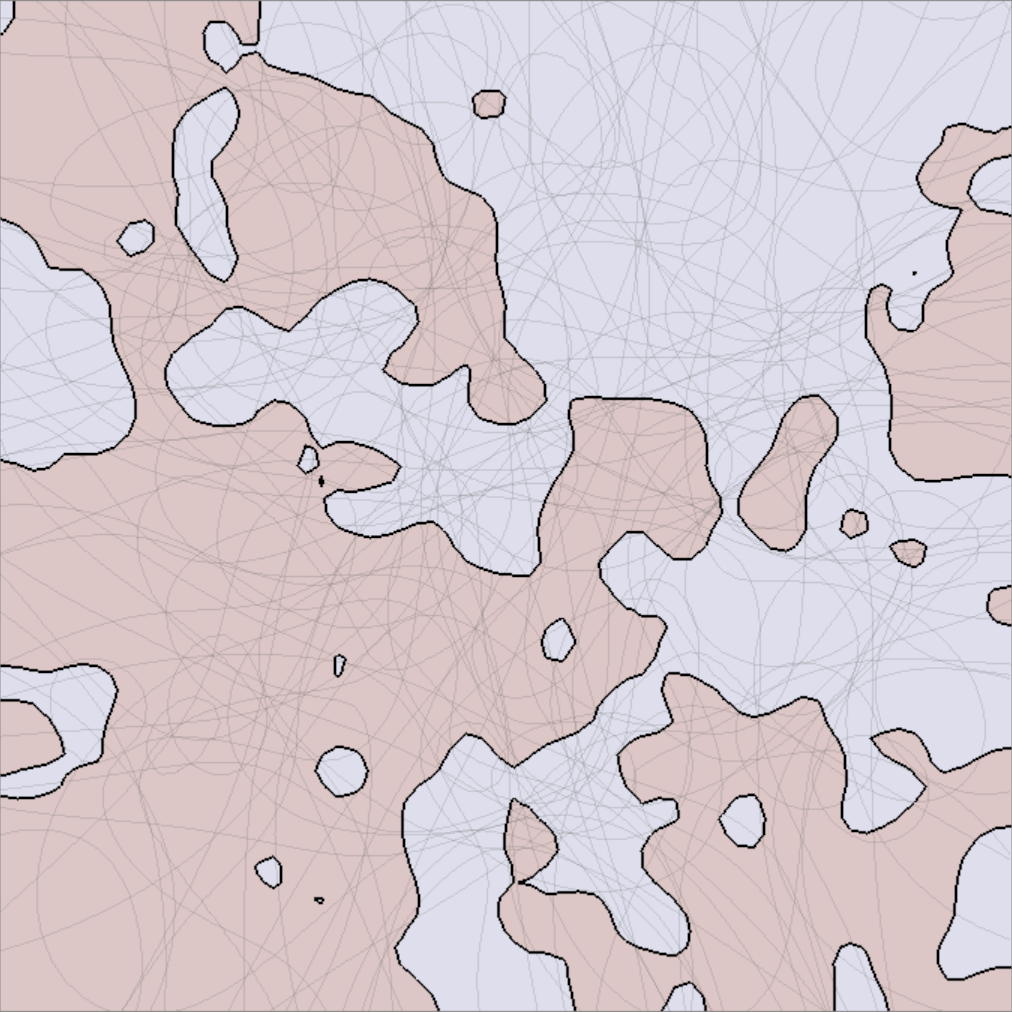
\includegraphics[width = 3 in]{1blur.png}
  \caption{The output of the Marching Squares algorithm: curvilinear, radial separation. 
Grid resolution is 64x64.
All contour sets have been drawn in transparent grey, with the exception of the average contour set, which is drawn in pure black.
}
\end{figure}







\begin{figure} 
\centering
  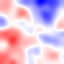
\includegraphics[width = 3 in]{image_avg_10blur.png}
  \caption{Bitmap image used as input to the Marching Squares algorithm.
Image size is 64x64.
Ten iterations of Gaussian blur have been used.
}
\end{figure}
	
\begin{figure} 
\centering
  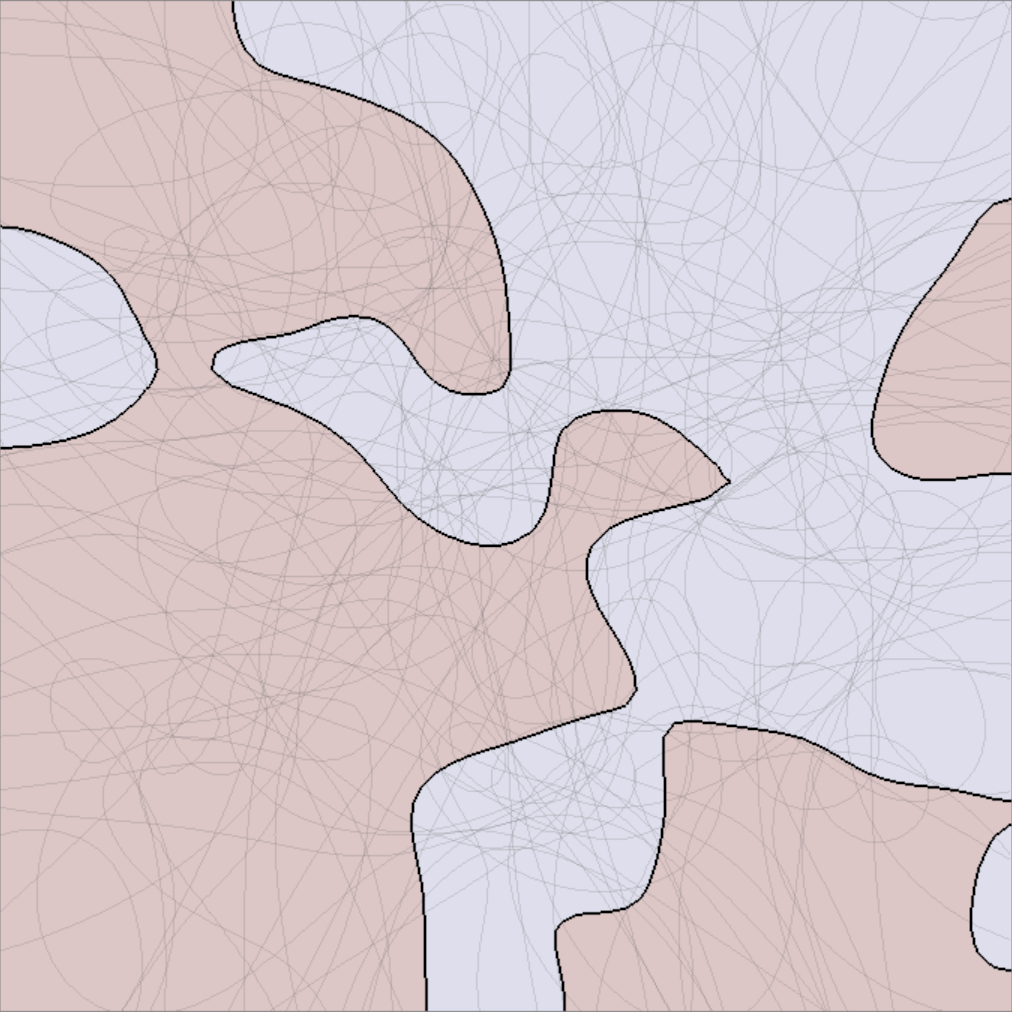
\includegraphics[width = 3 in]{10blur.png}
  \caption{The output of the Marching Squares algorithm: curvilinear, radial separation. 
Grid resolution is 64x64.
All contour sets have been drawn in transparent grey, with the exception of the average contour set, which is drawn in pure black.
}
\end{figure}





\end{document}









